\documentclass{beamer}
\usepackage[utf8]{inputenc}
\usepackage[croatian]{babel}
\mode<presentation>
{
  \usetheme{default}      
  \usecolortheme{default} 
  \usefonttheme{default}  
  \setbeamertemplate{navigation symbols}{}
  \setbeamertemplate{caption}[numbered]
} 

\title[]{Git vs Mercurial}
\author{Karlo Graf\newline Matej Katalinić\newline Vanja Ljubobratović}
\institute{Tehnički Fakultet, Sveučilište u Rijeci}

\begin{document}

\begin{frame}
  \titlepage
\end{frame}

% Uncomment these lines for an automatically generated outline.
%\begin{frame}{Outline}
%  \tableofcontents
%\end{frame}

\begin{frame}{Uvod}

\begin{itemize}
  \item U ovoj prezentaciji usporediti ćemo dva sustava za distibuirano upravljanje verzijama: Git i Mercurial
  \item Kreniti ćemo od osnovnih naredbi u Mercurialu te prinicipe njegova korištenja i kasnije ga usporediti sa Git-om
\end{itemize}

\vskip 1cm


\end{frame}

\begin{frame}{O sustavima za upravljanje verzijama}

Upravljanje verzijama podrazumijeva baratanje promjenama nad nekim skupom datoteka pamćenjem povijesti promjena. Spremište povijesti promjena nazivamo repozitorijem. Ovakvi sustavi se koriste jer nam uvelike olakšavaju rad na velikim i kompliciranim projektima, osobito ako radimo u timu. Neke od prednosti ovakvih sustava su:
\begin{itemize}
  \item Nemoramo se brinuti o imenima projekata (v1,v1.1,v1.2,v1...) jer za tim nema potrebe. Ti sustavi će sami za nas pratiti koja je koja verzija i nemoguće ih je slučajno zamijeniti.
  \item Olakšava komunikaciju između kolega jer si više nemoraju međusobno slati datoteke svaki put kada nešto novo dodaju nego se to jednostavno "gurne" u repozitorij i svi vide promjene te ih mogu preuzeti
\end{itemize}
\end{frame}
\begin{frame}{Naredbe u Mercurialu}
Naredbe u Gitu i Mercurialu su vrlo slične. Glavna razlika je naravno umjesto započivanja svake naredbe sa "git" u Gitu, u Mercurialu naredbe započinjemo sa "hg". Većinu naredbi koje imamo u gitu imamo i u Mercurialu samo sa malo drugčijom sintaksom(zapisom). Kao na primjer u gitu: "git remote add origin<server-url>" i u Mercurialu: "hg push <server-url>". Obje naredbe služe za povezivanje našeg lokalnog repozitorija na udaljeni server i kao što vidite razilika u sintaksi je velika. 

\end{frame}

\begin{frame}{Grane i Bookmarkovi}
Vrlo često na svom projektu želimo isprobati nešto novo, ali ne želimo to raditi na originalnoj verziji programa jer nismo sigurni što točno želimo i ako je to uopće moguće. U tom slučaju koristiti ćemo različite grane. Grane su kao što ime govori kada se granamo s glavnog projekta te radimo nešto neovisno o njemu. Kasnije te grane možemo spajati, brisati i još par stvari. No u Mercurialu nije točno tako. U Mercurialu su grane mnogo "skuplje" od grana u gitu. U gitu grana je pokazivač na određeni commit dok je u Mercurialu grana povezana sa commitom te se nemože brisati ni preimenovati. Zato se u Mercurialu mogu korisiti Bookmarkovi. Bookmarkovi rade na istomp principu kao i grane u gitu.
\end{frame}

\begin{frame}{Git vs Mercurial Workflow}
\begin{figure}
    \centering
    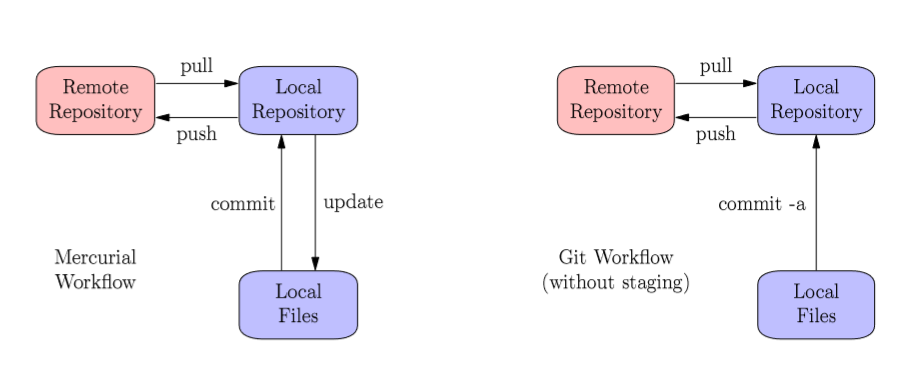
\includegraphics[width = 310px]{workflows.png}
    \label{fig:my_label}
\end{figure}
\end{frame}

\begin{frame}{Upotreba Git-a}
\begin{itemize}
    \item Netflix
    \item Reddit 
    \item Lyft
    \item StackShare
    \item Quora
\end{itemize}
\end{frame}

\begin{frame}{Upotreba Mercurial-a}
\begin{itemize}
    \item Bitbucket
    \item Performance Assessment Network (PAN)
    \item Deveo
    \item inFeedo
    \item emotion.me
\end{itemize}
\end{frame}
\end{document}

